\section{Antenna Design 3 -- Allan}
In this section, the results from Section~\ref{sec:tech_sol_ant3} will be repeated, having the phone in data mode, play mode, and talk mode\fixme{Use correct terms!}. Furthermore, the maximum SAR value, recorded in the users head, will be simulated. The antenna positions, for each use case, are shown in Figure~\ref{fig:ant3_positions}.

\begin{figure}[htbp]
    \centering
    \begin{subfigure}[b]{0.24\linewidth}
        \centering
        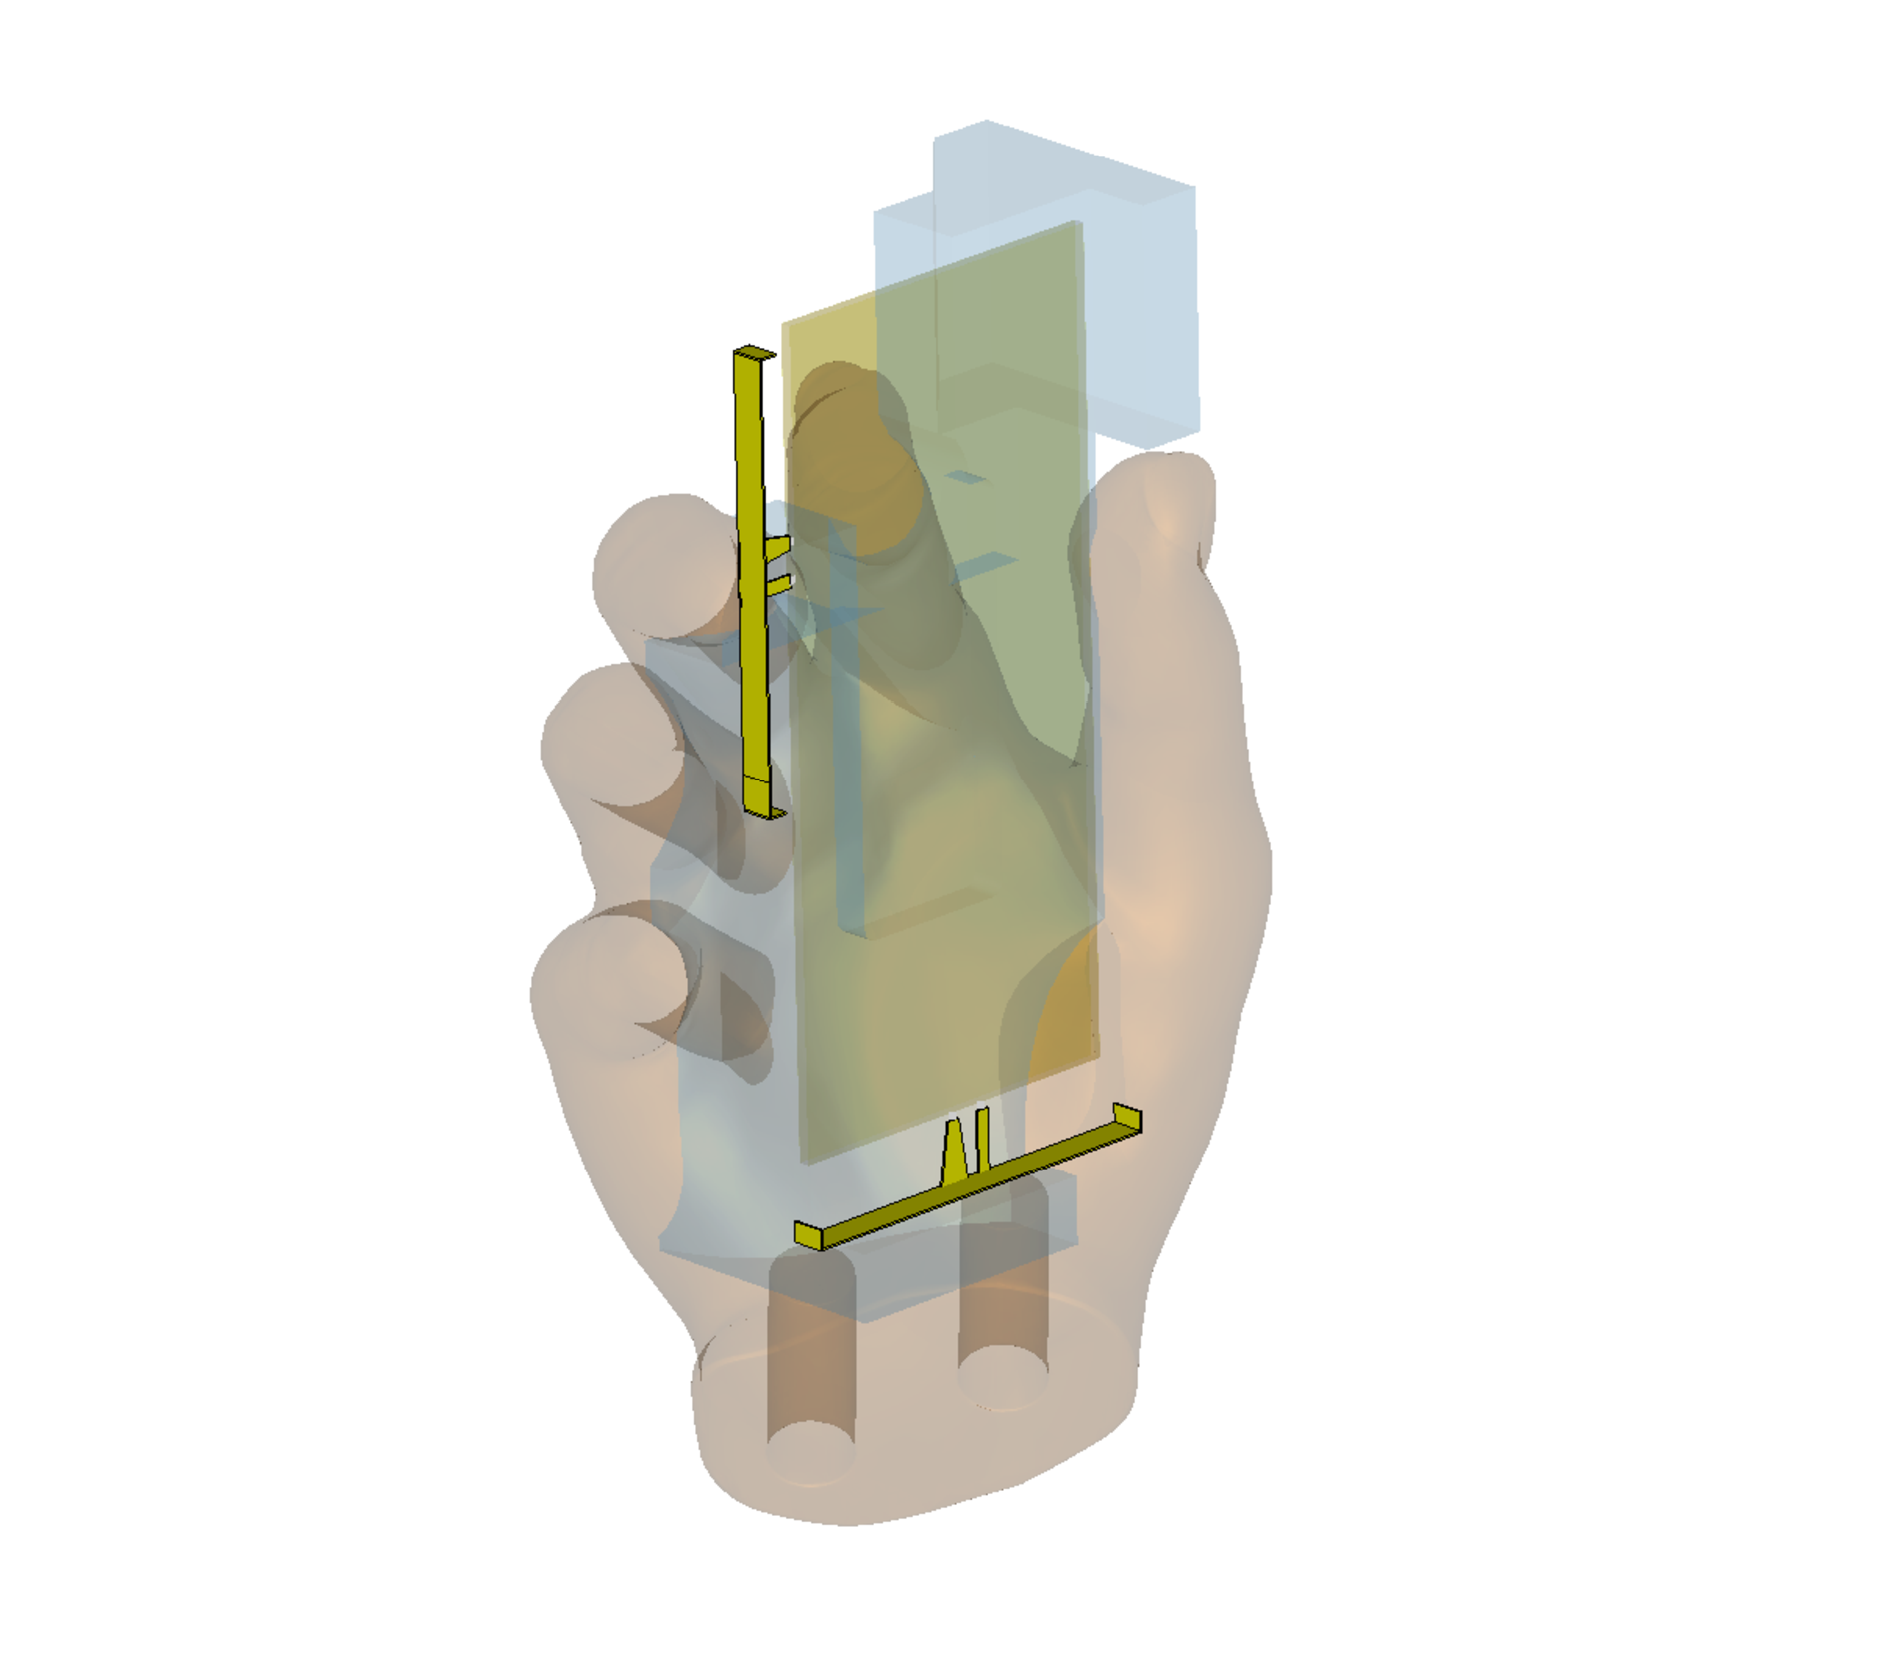
\includegraphics[width=\linewidth,height=4cm,keepaspectratio]{img/tech_sol/nonresonant/simulation/data_mode/3d}
        \caption{Data mode.}
    \end{subfigure}
    \begin{subfigure}[b]{0.24\linewidth}
        \centering
        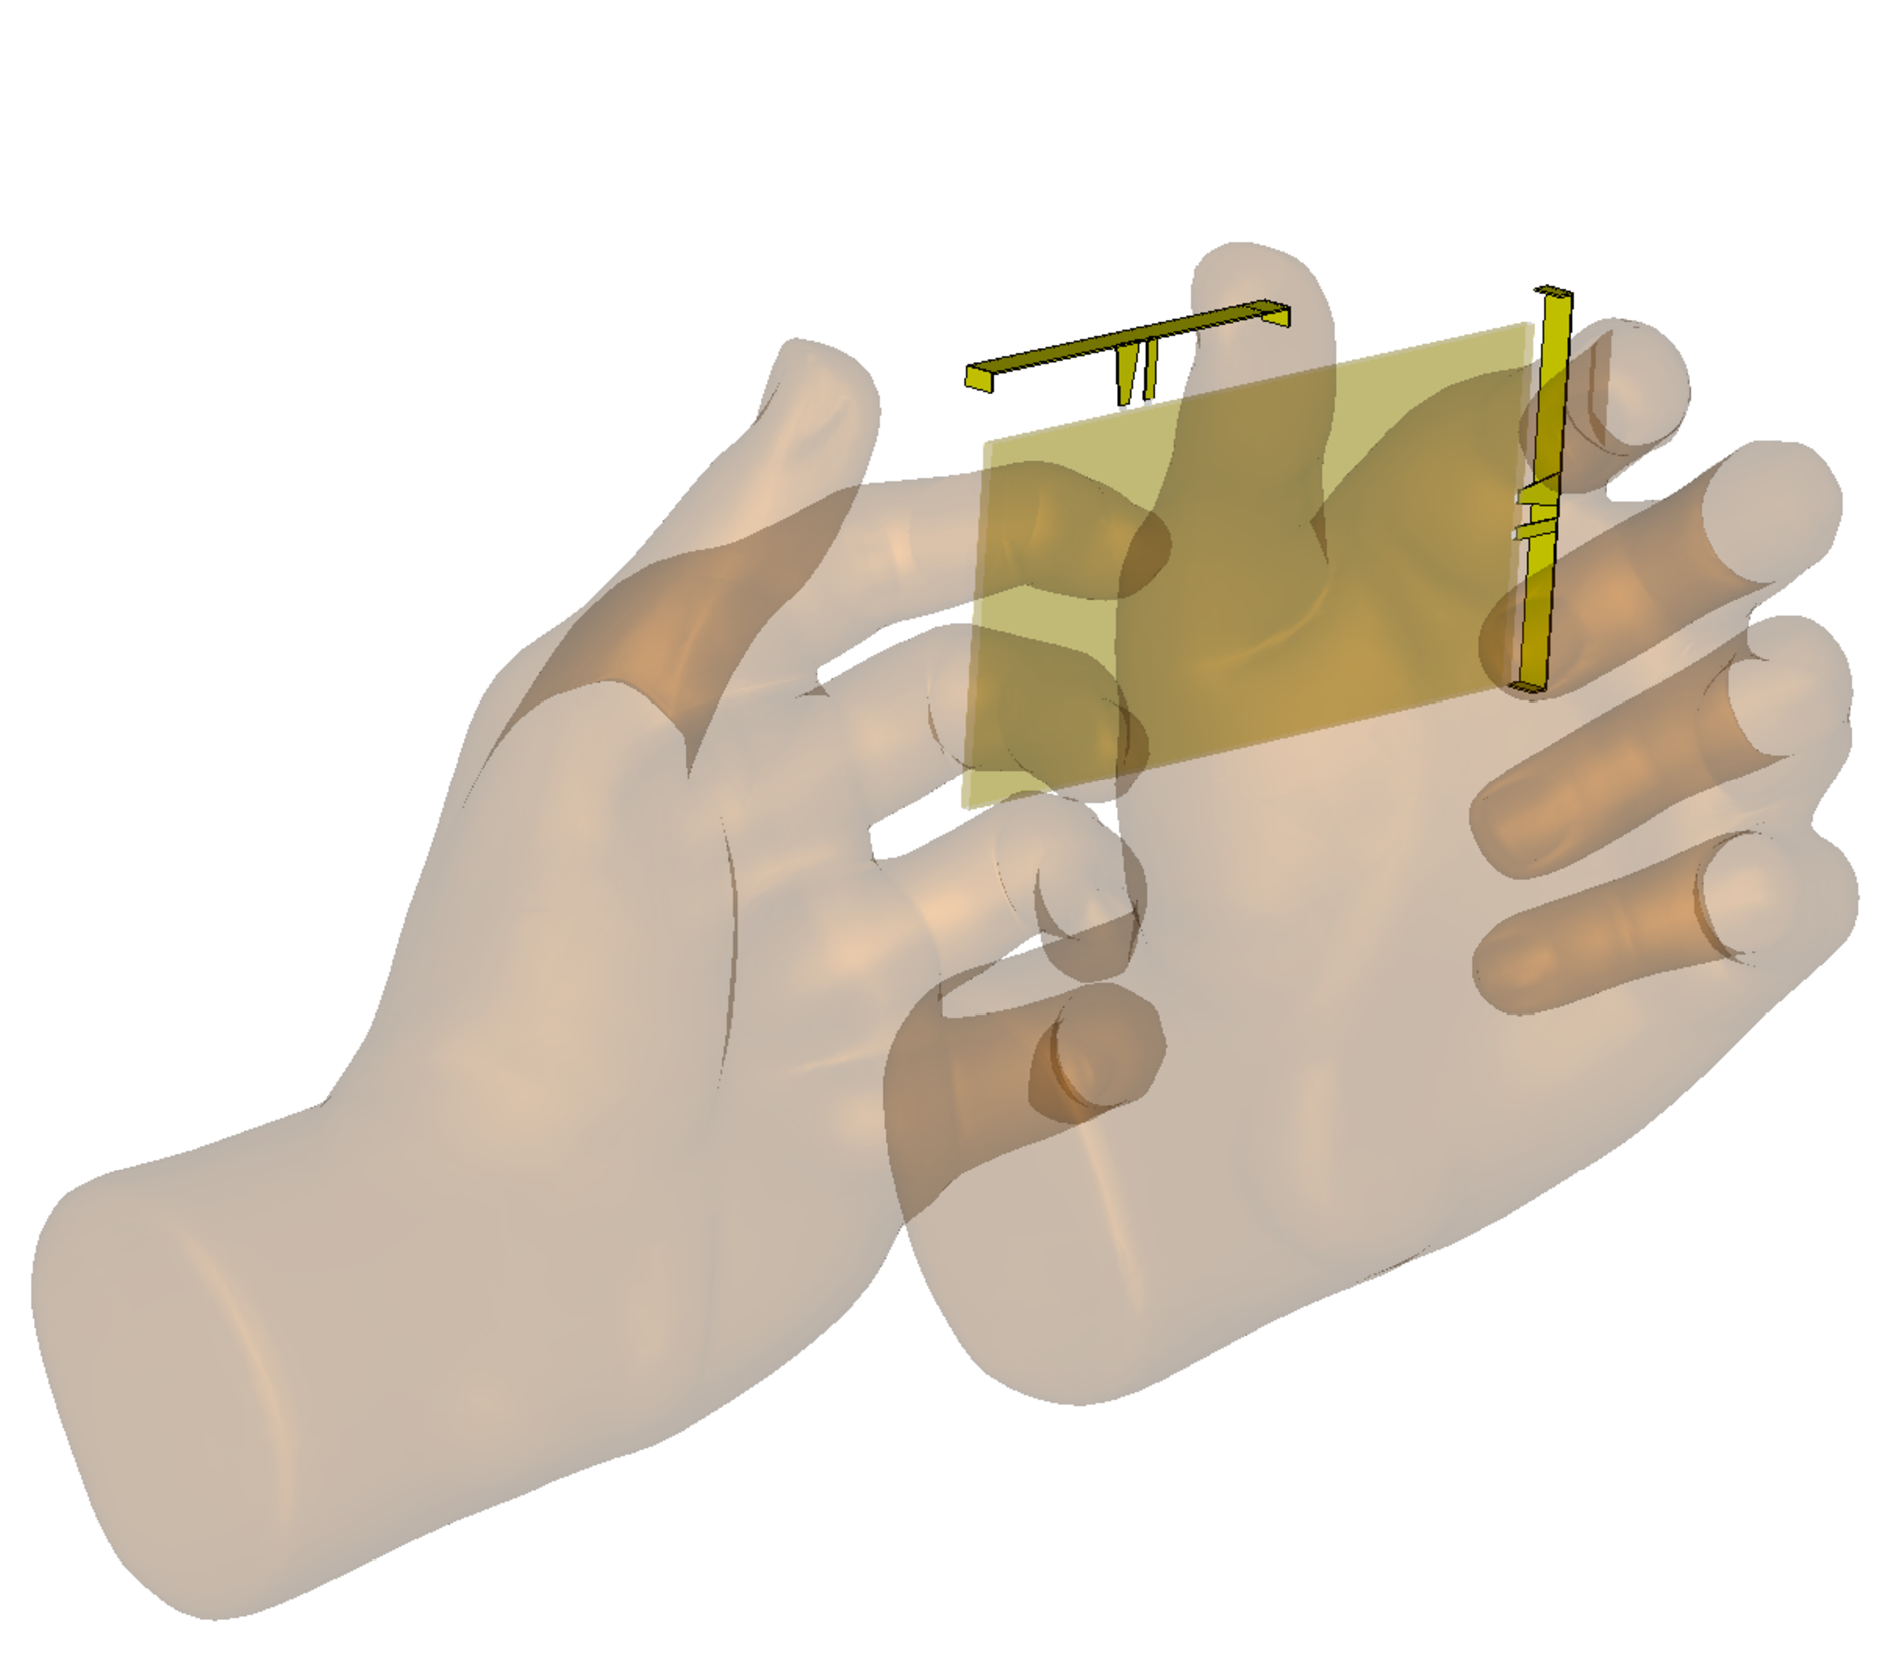
\includegraphics[width=\linewidth,height=4cm,keepaspectratio]{img/tech_sol/nonresonant/simulation/play_mode/3d}
        \caption{Play mode.}
    \end{subfigure}
    \begin{subfigure}[b]{0.24\linewidth}
        \centering
        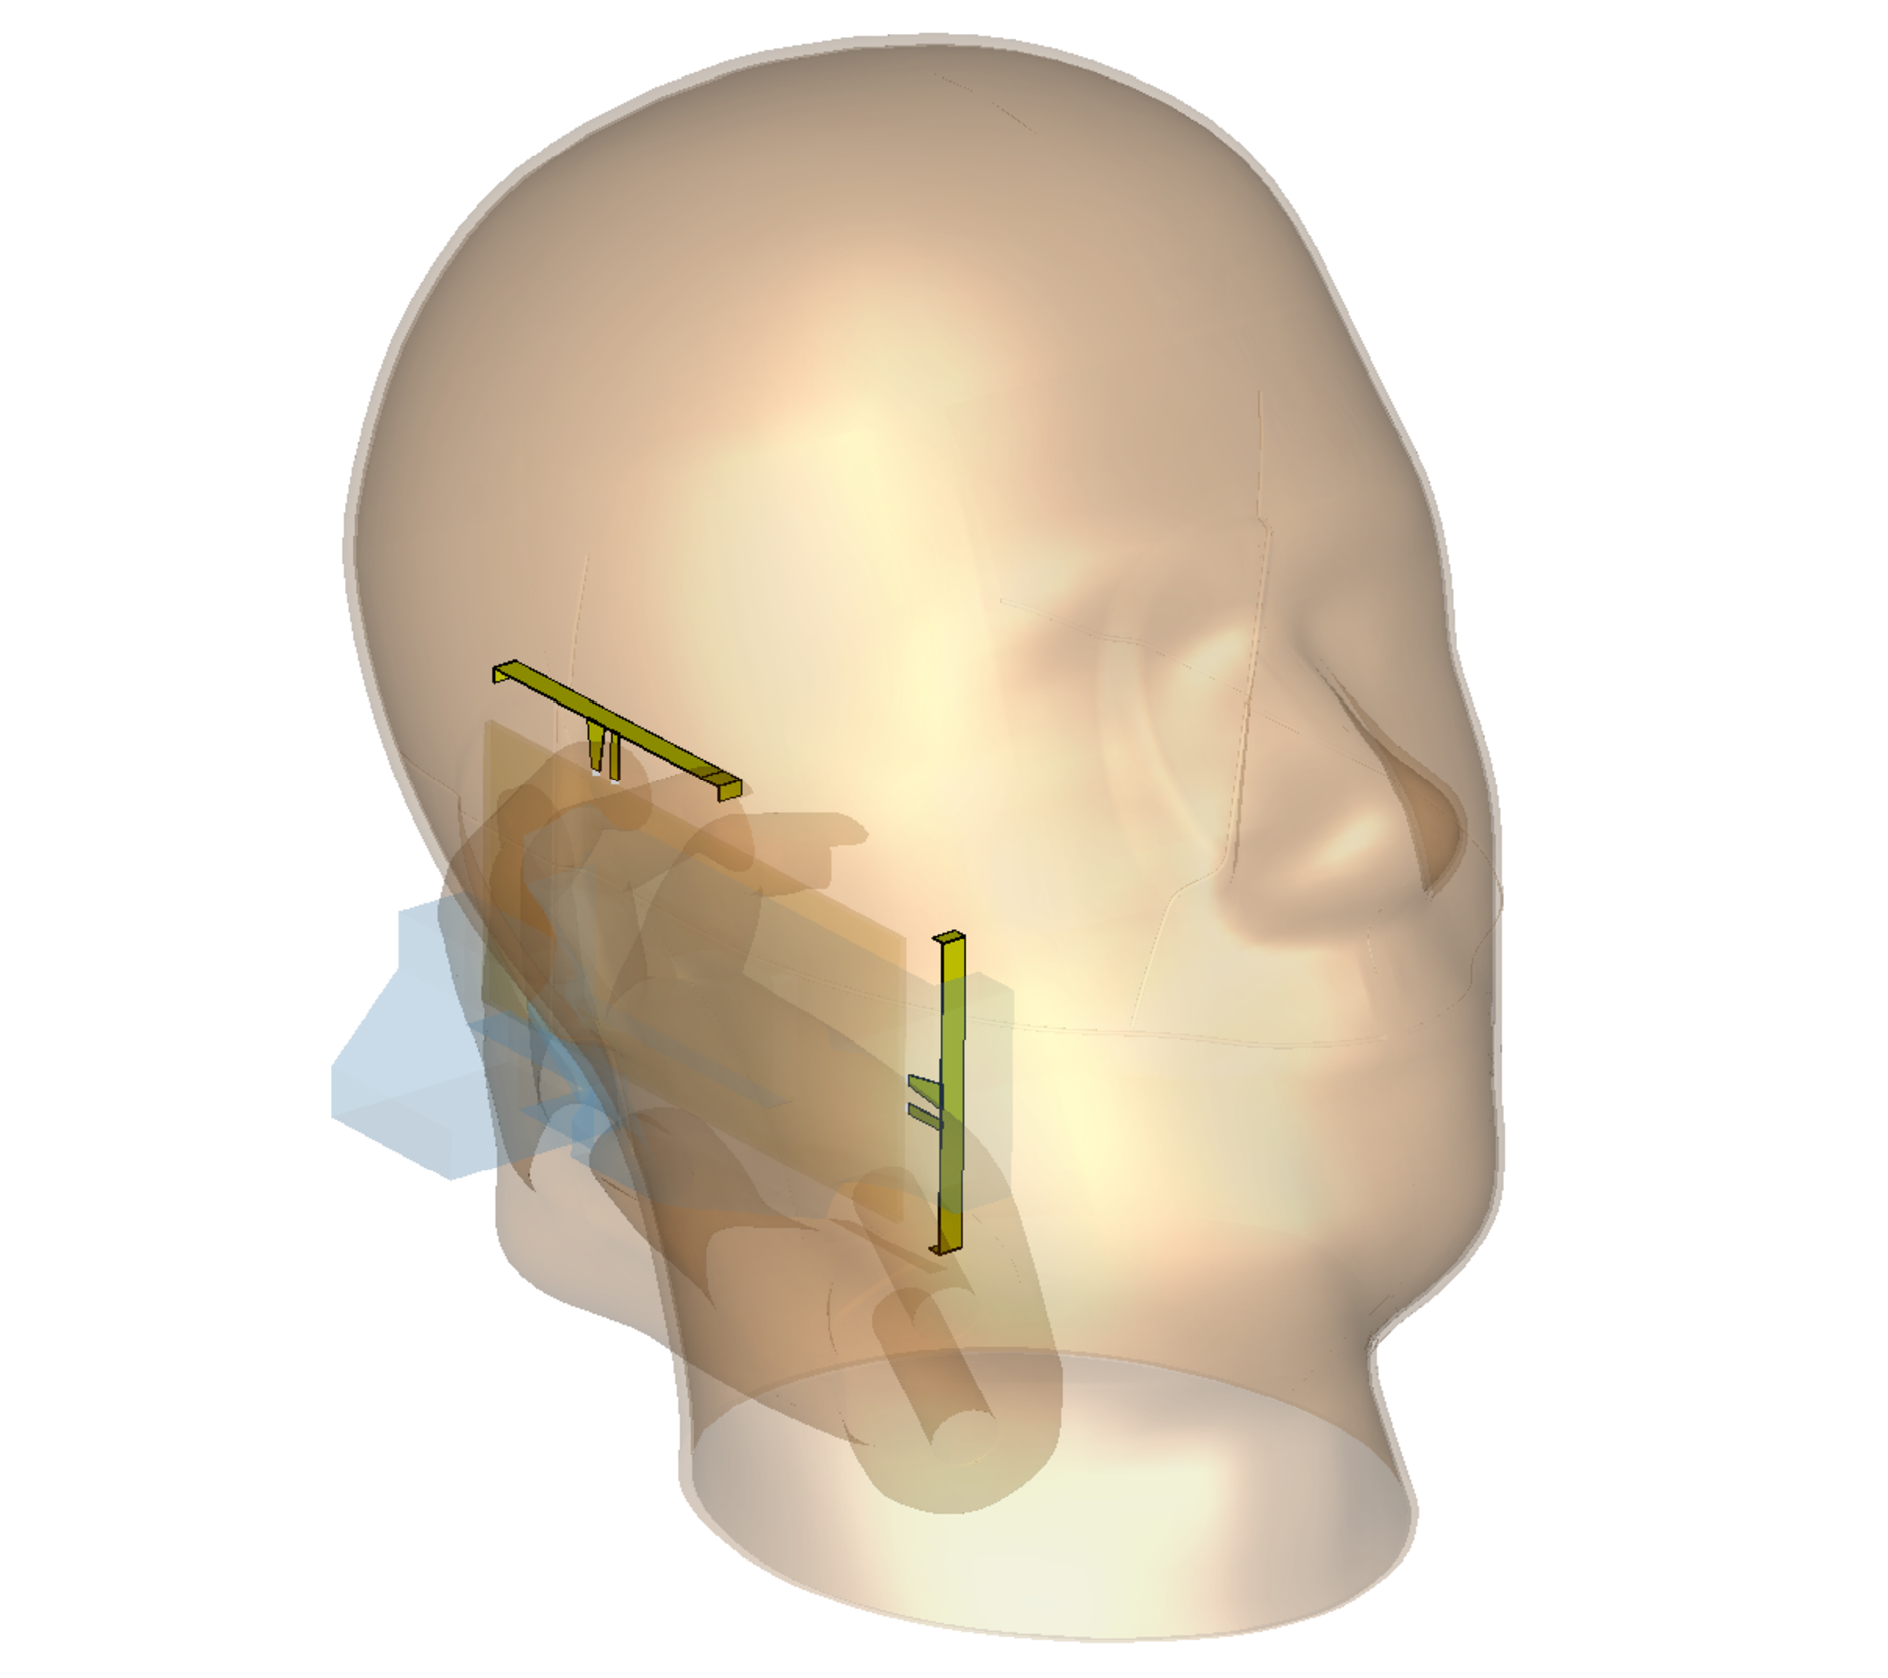
\includegraphics[width=\linewidth,height=4cm,keepaspectratio]{img/tech_sol/nonresonant/simulation/talk_mode/3d}
        \caption{Talk mode.}
    \end{subfigure}
    \begin{subfigure}[b]{0.24\linewidth}
        \centering
        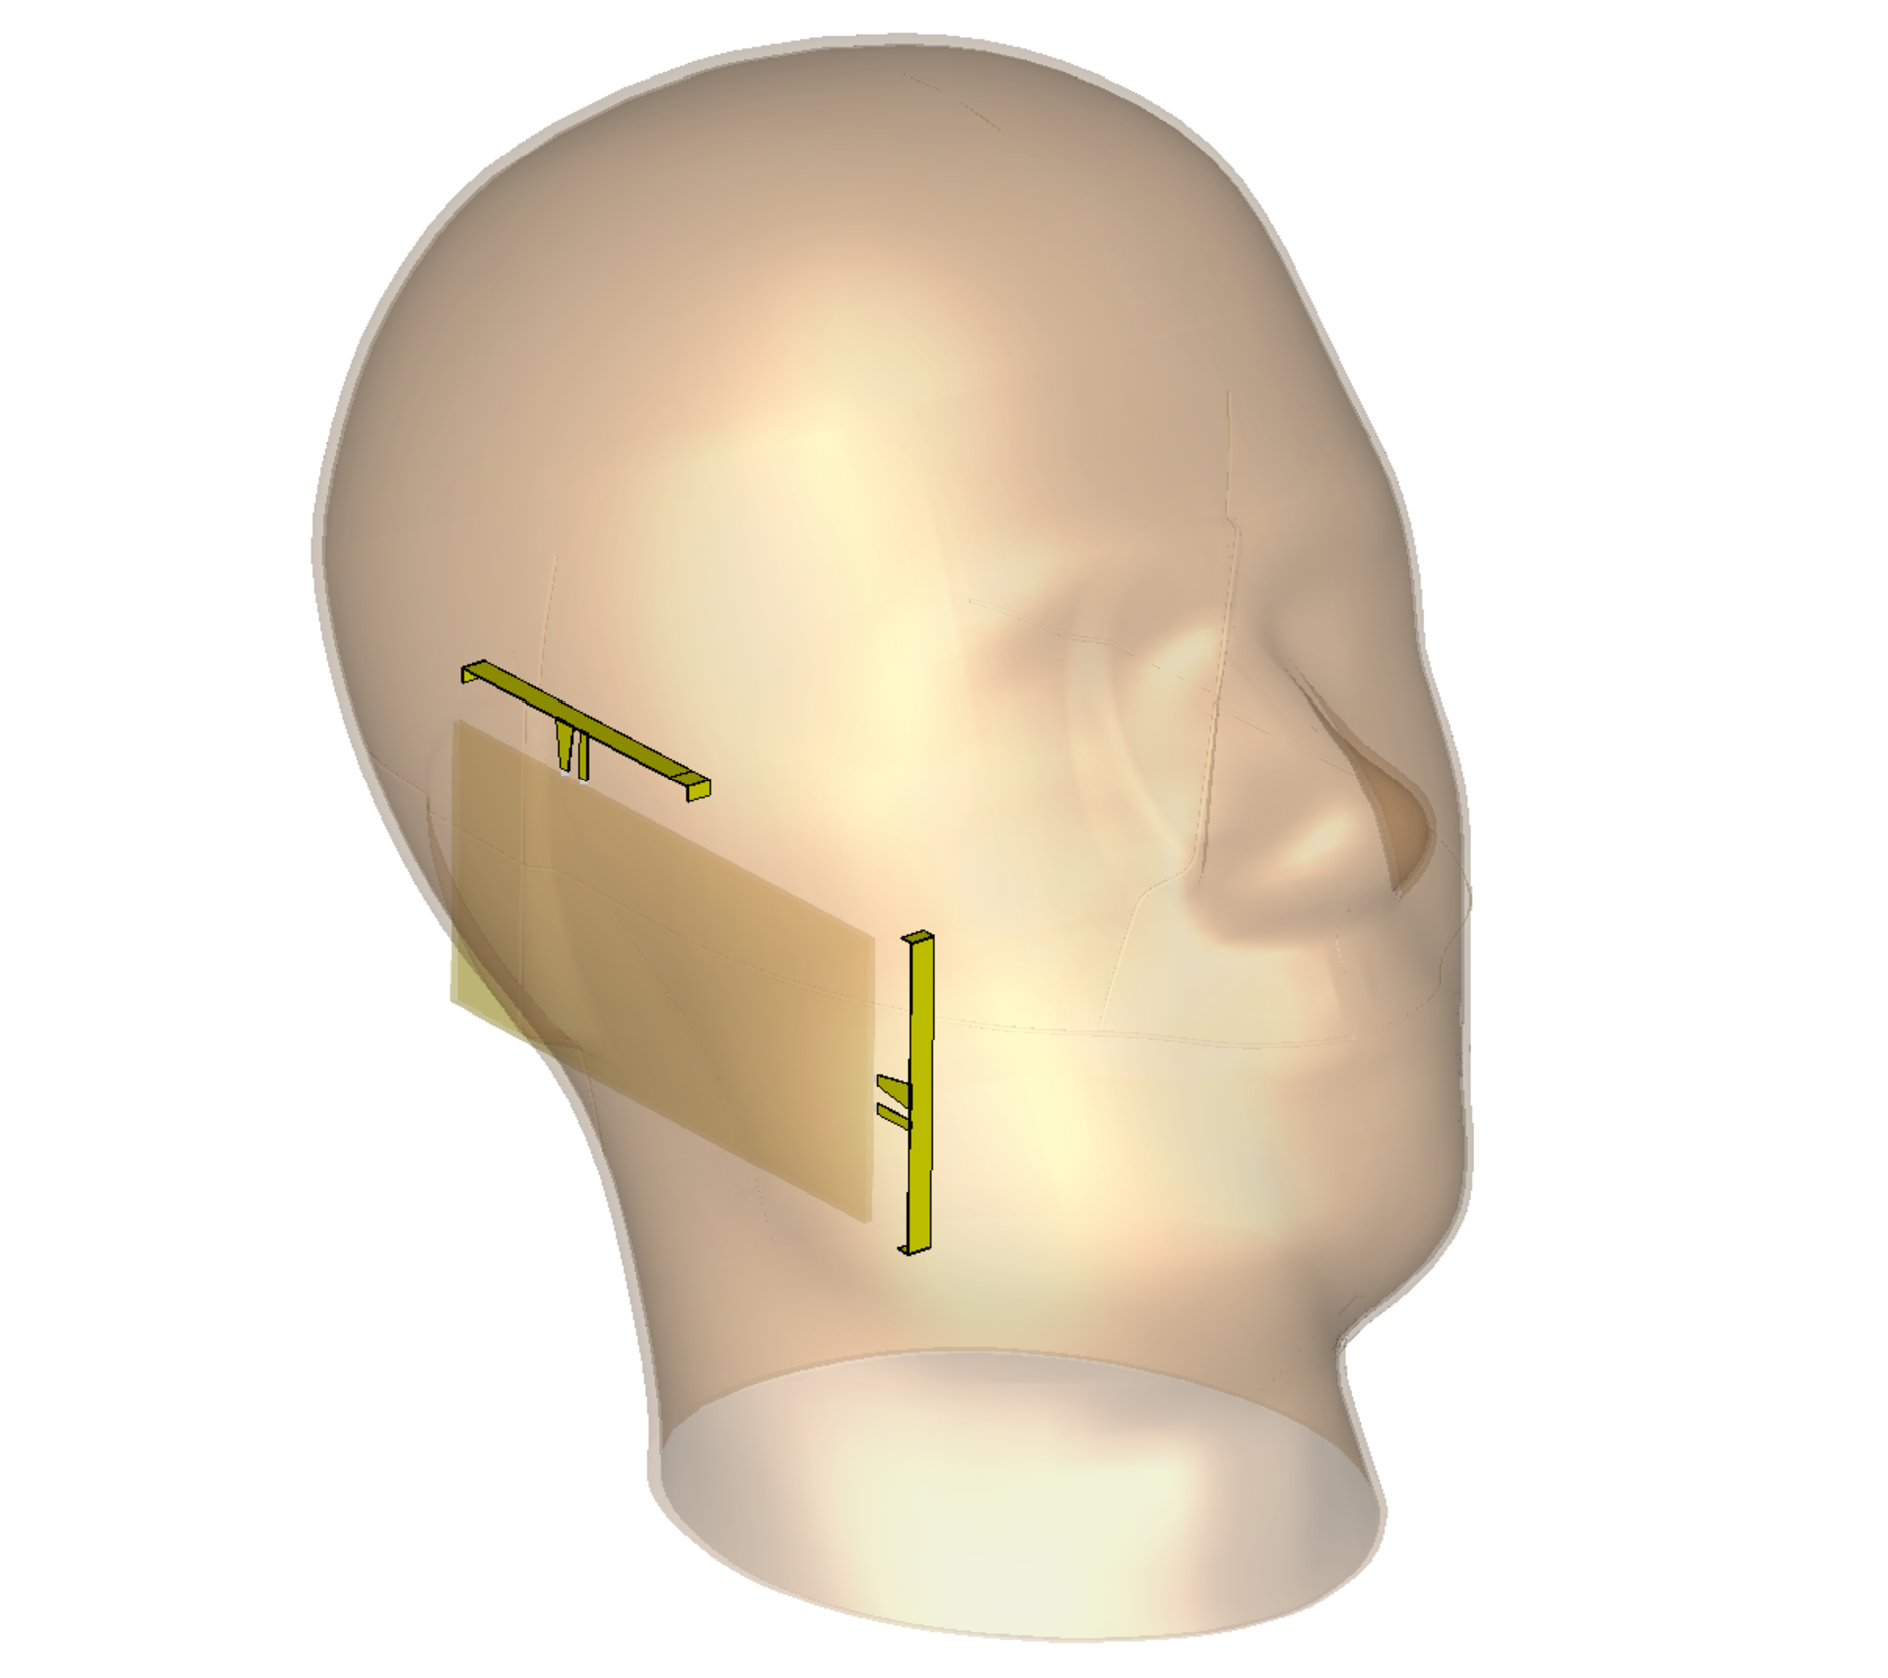
\includegraphics[width=\linewidth,height=4cm,keepaspectratio]{img/tech_sol/nonresonant/simulation/sar/3d}
        \caption{SAR.}
    \end{subfigure}
    \caption{Antenna position for each user effect simulation.}
    \label{fig:ant3_positions}
\end{figure}

\FloatBarrier
\subsection{Data Mode}
Figure~\ref{fig:ant3_sparam_data} shows the S-parameters with the tunabale capacitors set to their maxima. Such both the top and side antennas have been tuned down to the lowest possible frequency. It is seen that the top antenna covers most of the band from \SI{700}{MHz} to \SI{960}{MHz}, with a reflection coefficient below \SI{-6}{dB}. The side antenna is however very narrow band, and must be tuned in order to cover all the low bands. It is also seen that the side antenna does not cover the entire high band, when tuned down to the lowest. 

The S-parameters, when sweeping the tunable capacitors, are shown in Figure~\ref{fig:ant3_sparam_sweep_data}. The maximum impedance-bandwidths are summed up in Table~\ref{tab:bw_sol3data}. From this it is again clear that only the top antenna is able to cover the high end of the low band. Both antennas should be able to cover the entire high band at \SI{6}{dB} return loss.

The correlation between the antennas, when sweeping the tunable capacitors, are shown in Figure~\ref{fig:corr_sol3_data}. The correlation is, for frequencies above \SI{700}{MHz}, below 0.4 when sweeping the top and side antenna. For the high band the correlation is significantly lower, which is also to be expected. The correlation has dropped a lot from the free-space simulation in Figure~\ref{fig:corr_sol3}.

The efficiencies for each antenna, when sweeping the tuning capacitors, are shown in Figure~\ref{fig:eff_sol3data}. It is seen that the efficiency, generally, has decreased from the free space simulation in Chapter~\ref{cha:nousersim}. At  \SI{-3}{dB} efficiency, there is no bandwidth left. At \SI{-6}{dB} all bands are covered. The efficiency in the high band is generally higher than in the low band.

\begin{figure}[htbp]
    \centering
    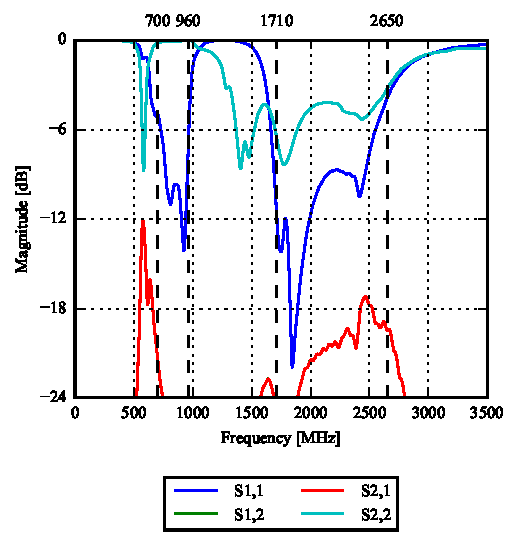
\includegraphics{img/tech_sol/nonresonant/simulation/data_mode/s_params_cMax.pdf}
    \caption{The antenna in data mode. S-parameters with both tuning capacitors fixed at \SI{2.9}{pF}.}
    \label{fig:ant3_sparam_data}
\end{figure}

\begin{table}[htbp]
    \centering
    \begin{tabular}{|l|l|r|r|r|}
        \hline
        Antenna & Band & Start [MHz] & Stop [MHz] & Bandwidth [MHz] \\
        \hline
        Top     & Low  & 570         & 2583       & 2013 \\
        Side    & Low  & 779         & 891        & 112  \\
        \hline
        Top     & High & 570         & 2583       & 2013 \\
        Side    & High & 1506        & 2623       & 1117 \\
        \hline
    \end{tabular}
    \caption{The antenna in data mode. Maximum bandwidth obtained in the low and high band for the top and the side antenna, respectively.}
    \label{tab:bw_sol3data}
\end{table}

\begin{figure}[htbp]
   \begin{subfigure}[b]{0.49\linewidth}
        \centering
        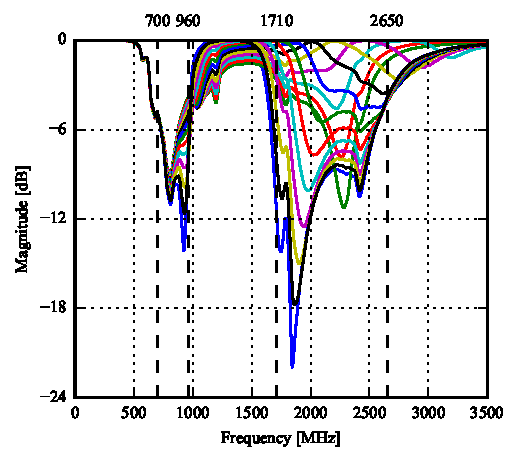
\includegraphics{img/tech_sol/nonresonant/simulation/data_mode/s11_top_sweep.pdf}
        \caption{$S_{11}$, sweeping $C_{l3}$ and fixing $s\_C_{h1}$.}
    \end{subfigure}
    \hfill
    \begin{subfigure}[b]{0.49\linewidth}
        \centering
        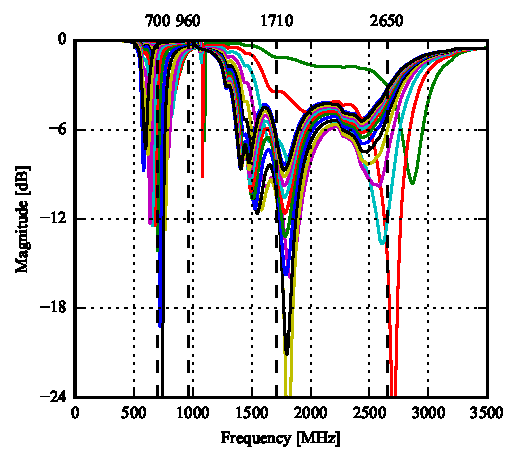
\includegraphics{img/tech_sol/nonresonant/simulation/data_mode/s22_side_sweep.pdf}
        \caption{$S_{22}$, sweeping $C_{l3}$ and fixing $s\_C_{h1}$.}
    \end{subfigure}
    \\
    \begin{subfigure}[b]{0.49\linewidth}
        \centering
        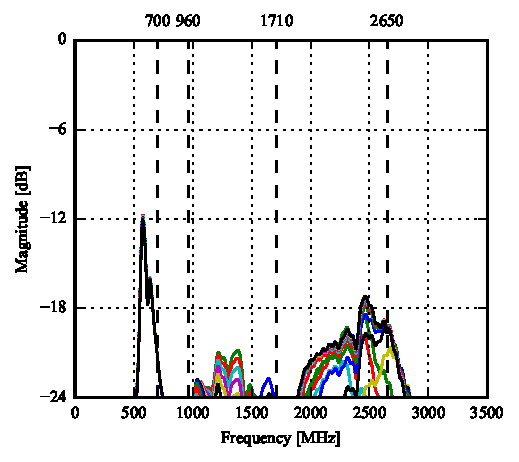
\includegraphics{img/tech_sol/nonresonant/simulation/data_mode/s12_top_sweep.pdf}
        \caption{$S_{21}$, sweeping $C_{l3}$ and fixing $s\_C_{h1}$.}
    \end{subfigure}
    \hfill
    \begin{subfigure}[b]{0.49\linewidth}
        \centering
        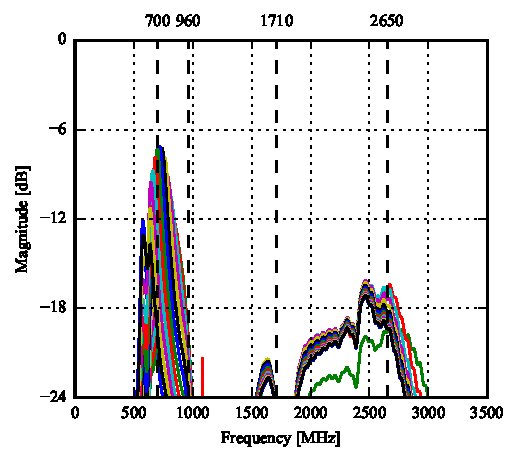
\includegraphics{img/tech_sol/nonresonant/simulation/data_mode/s21_side_sweep.pdf}
        \caption{$S_{21}$, sweeping $s\_C_{h1}$ and fixing $C_{l3}$.}
    \end{subfigure}
    \caption{The antenna in data mode. Parameter sweep for tuning the shunt capacitor of each antenna, $C_{l3}$ and $s\_C_{h1}$ for port 1 and 2, respectively. Port 1 is the top antenna and port 2 is the side antenna.}
    \label{fig:ant3_sparam_sweep_data}
\end{figure}

% Correlation
\begin{figure}[htbp]
    \centering
    \begin{subfigure}{0.49\linewidth}
        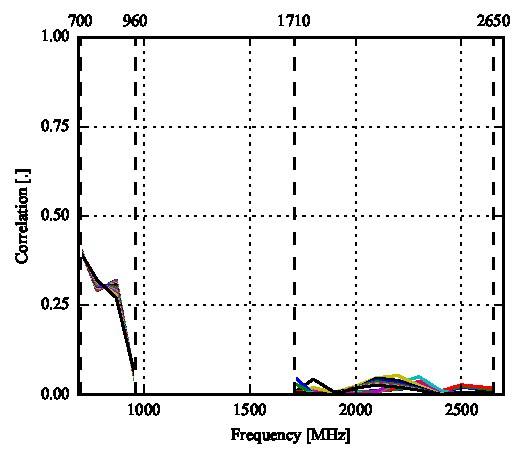
\includegraphics{img/tech_sol/nonresonant/simulation/data_mode/sweep_top_corr}
        \caption{Sweeping $C_{l3}$ and fixing $s\_C_{h1}$.}
    \end{subfigure}
    \hfill
    \begin{subfigure}{0.49\linewidth}
        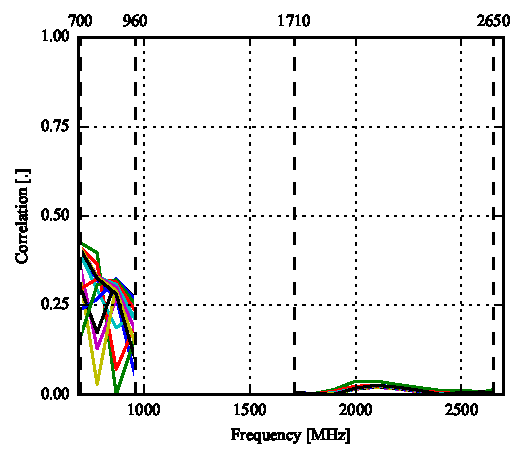
\includegraphics{img/tech_sol/nonresonant/simulation/data_mode/sweep_side_corr}
        \caption{Sweeping $s\_C_{h1}$ and fixing $C_{l3}$.}
    \end{subfigure}
    \caption{The antenna in data mode. Correlation between antennas then sweeping tuning capacitors. Here, $C_{l3}$ and $s\_C_{h1}$ are the tuning capacitor for the top and side antenna, respectively.}
    \label{fig:corr_sol3_data}
\end{figure}

% Efficiency
\begin{figure}[htbp]
    \centering
    \begin{subfigure}{0.49\linewidth}
        \centering
        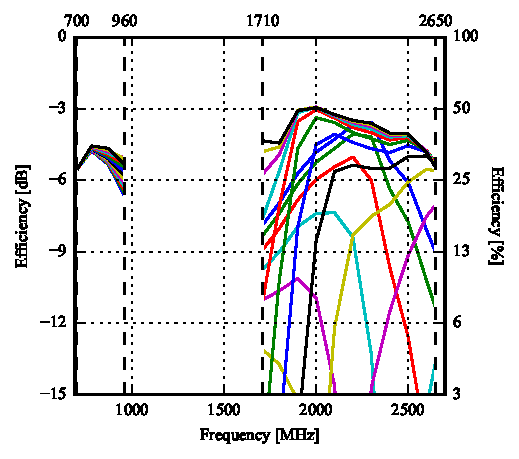
\includegraphics{img/tech_sol/nonresonant/simulation/data_mode/EffSweepAC1/efficiency-ac1-top}
        \caption{Top antenna. Sweeping $C_{l3}$, fixing $s\_C_{h1}$.}
    \end{subfigure}
    \hfill
    \begin{subfigure}{0.49\linewidth}
        \centering
        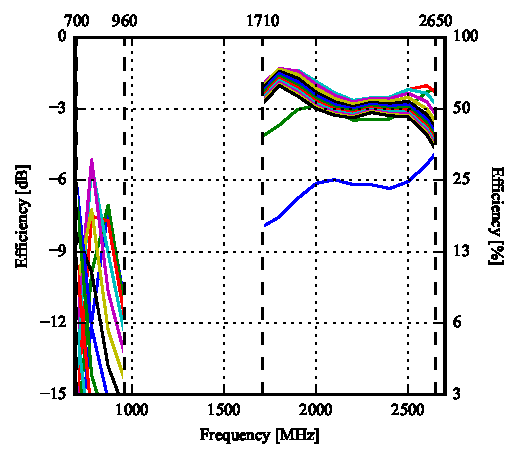
\includegraphics{img/tech_sol/nonresonant/simulation/data_mode/EffSweepAC2/efficiency-ac2-side}
        \caption{Side antenna. Sweeping $s\_C_{h1}$, fixing $C_{l3}$.}
    \end{subfigure}
    \caption{The antenna in data mode. Efficiency for each antenna when sweeping the tuning capacitors. Here, $C_{l3}$ and $s\_C_{h1}$ are the tuning capacitor for the top and side antenna, respectively.}
    \label{fig:eff_sol3data}
\end{figure}


\FloatBarrier
\subsection{Play Mode}
Figure~\ref{fig:ant3_sparam_play} shows the S-parameters with the tunabale capacitors set to their maxima. Such both the top and side antennas have been tuned down to the lowest possible frequency. It is seen that the top antenna covers most of the band from \SI{700}{MHz} to \SI{960}{MHz}, with a reflection coefficient below \SI{-6}{dB}. The side antenna is however very narrow band, and must be tuned in order to cover all the low bands. It is also seen that the side antenna does not cover the entire high band, when tuned down to the lowest. 

The S-parameters, when sweeping the tunable capacitors, are shown in Figure~\ref{fig:ant3_sparam_sweep_play}. The maximum impedance-bandwidths are summed up in Table~\ref{tab:bw_sol3data}. From this it is again clear that only the top antenna is able to cover the high end of the low band. Both antennas should be able to cover the entire high band at \SI{6}{dB} return loss.

The correlation between the antennas, when sweeping the tunable capacitors, are shown in Figure~\ref{fig:corr_sol3_play}. The correlation is, for frequencies above \SI{700}{MHz}, below 0.4 when sweeping the top and side antenna. For the high band the correlation is significantly lower, which is also to be expected. Again the correlation has dropped a lot from the free-space simulation in Figure~\ref{fig:corr_sol3}.

The efficiencies for each antenna, when sweeping the tuning capacitors, are shown in Figure~\ref{fig:eff_sol3play}. It is seen that the efficiency, generally, has decreased from the free space simulation in Chapter~\ref{cha:nousersim} and also lower than the data mode. At \SI{-3}{dB} efficiency, there is no bandwidth left. At \SI{-6}{dB} most of the bands are covered.


\begin{figure}[htbp]
    \centering
    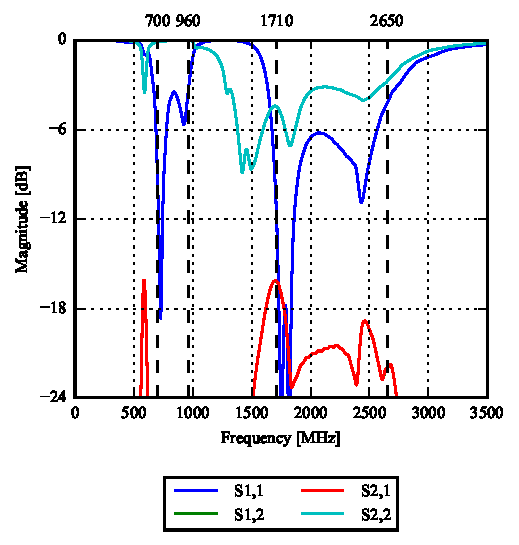
\includegraphics{img/tech_sol/nonresonant/simulation/play_mode/s_params_cMax.pdf}
    \caption{The antenna in play mode. S-parameters with both tuning capacitors fixed at \SI{2.9}{pF}.}
    \label{fig:ant3_sparam_play}
\end{figure}

\begin{table}[htbp]
    \centering
    \begin{tabular}{|l|l|r|r|r|}
        \hline
        Antenna & Band & Start [MHz] & Stop [MHz] & Bandwidth [MHz] \\
        \hline
        Top     & Low  & 629         & 928        & 299  \\
        Side    & Low  & 780         & 881        & 101  \\
        \hline
        Top     & High & 1379        & 2703       & 1324 \\
        Side    & High & 1388        & 2559       & 1171 \\
        \hline
    \end{tabular}
    \caption{The antenna in play mode. Maximum bandwidth obtained in the low and high band for the top and the side antenna, respectively. The bandwidth for the side antennas high band is ignoring the slight rise above \SI{-6}{dB} in the middle of the high band.}
    \label{tab:bw_sol3play}
\end{table}

\begin{figure}[htbp]
   \begin{subfigure}[b]{0.49\linewidth}
        \centering
        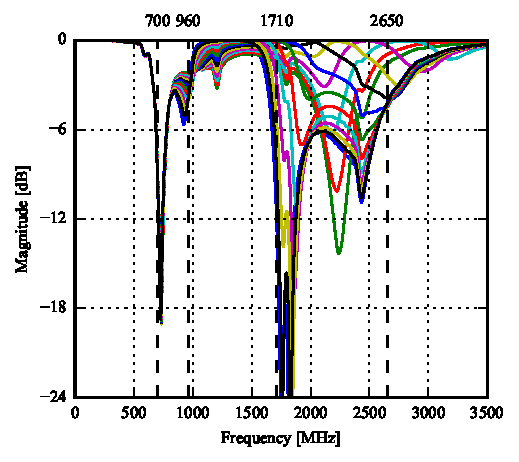
\includegraphics{img/tech_sol/nonresonant/simulation/play_mode/s11_top_sweep.pdf}
        \caption{$S_{11}$, sweeping $C_{l3}$ and fixing $s\_C_{h1}$.}
    \end{subfigure}
    \hfill
    \begin{subfigure}[b]{0.49\linewidth}
        \centering
        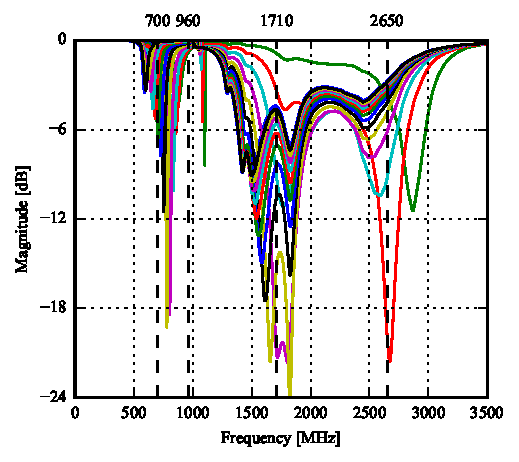
\includegraphics{img/tech_sol/nonresonant/simulation/play_mode/s22_side_sweep.pdf}
        \caption{$S_{22}$, sweeping $C_{l3}$ and fixing $s\_C_{h1}$.}
    \end{subfigure}
    \\
    \begin{subfigure}[b]{0.49\linewidth}
        \centering
        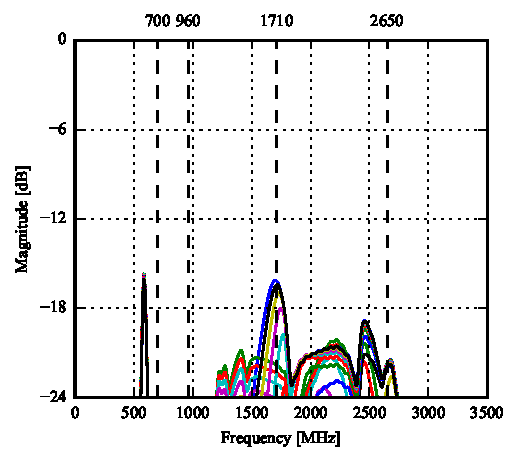
\includegraphics{img/tech_sol/nonresonant/simulation/play_mode/s12_top_sweep.pdf}
        \caption{$S_{21}$, sweeping $C_{l3}$ and fixing $s\_C_{h1}$.}
    \end{subfigure}
    \hfill
    \begin{subfigure}[b]{0.49\linewidth}
        \centering
        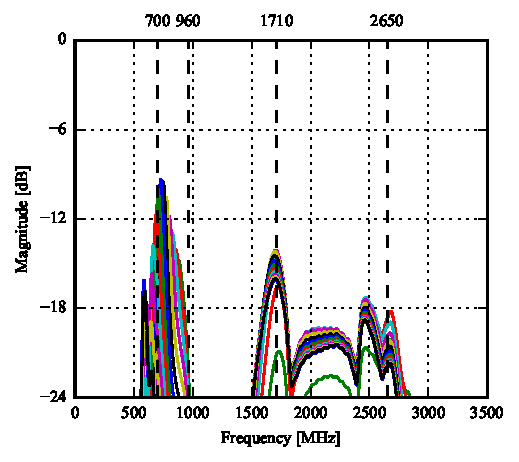
\includegraphics{img/tech_sol/nonresonant/simulation/play_mode/s21_side_sweep.pdf}
        \caption{$S_{21}$, sweeping $s\_C_{h1}$ and fixing $C_{l3}$.}
    \end{subfigure}
    \caption{The antenna in play mode. Parameter sweep for tuning the shunt capacitor of each antenna, $C_{l3}$ and $s\_C_{h1}$ for port 1 and 2, respectively. Port 1 is the top antenna and port 2 is the side antenna.}
    \label{fig:ant3_sparam_sweep_play}
\end{figure}

% Correlation
\begin{figure}[htbp]
    \centering
    \begin{subfigure}{0.49\linewidth}
        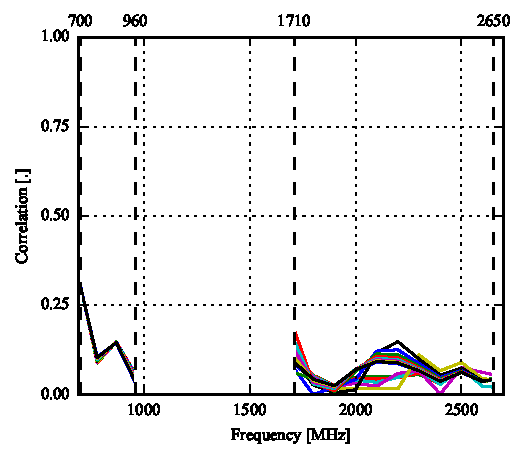
\includegraphics{img/tech_sol/nonresonant/simulation/play_mode/sweep_top_corr}
        \caption{Sweeping $C_{l3}$ and fixing $s\_C_{h1}$.}
    \end{subfigure}
    \hfill
    \begin{subfigure}{0.49\linewidth}
        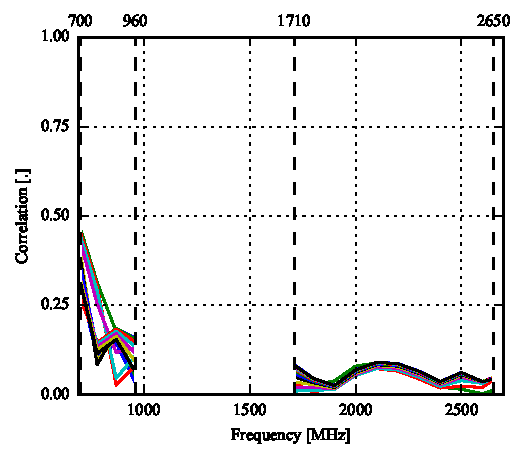
\includegraphics{img/tech_sol/nonresonant/simulation/play_mode/sweep_side_corr}
        \caption{Sweeping $s\_C_{h1}$ and fixing $C_{l3}$.}
    \end{subfigure}
    \caption{The antenna in play mode. Correlation between antennas then sweeping tuning capacitors. Here, $C_{l3}$ and $s\_C_{h1}$ are the tuning capacitor for the top and side antenna, respectively.}
    \label{fig:corr_sol3_play}
\end{figure}

% Efficiency
\begin{figure}[htbp]
    \centering
    \begin{subfigure}{0.49\linewidth}
        \centering
        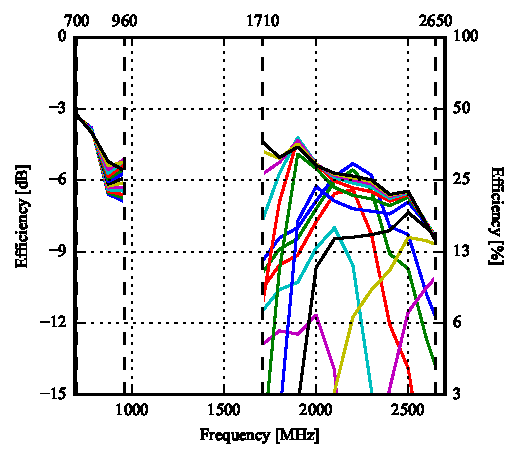
\includegraphics{img/tech_sol/nonresonant/simulation/play_mode/EffSweepAC1/efficiency-ac1-top}
        \caption{Top antenna. Sweeping $C_{l3}$, fixing $s\_C_{h1}$.}
    \end{subfigure}
    \hfill
    \begin{subfigure}{0.49\linewidth}
        \centering
        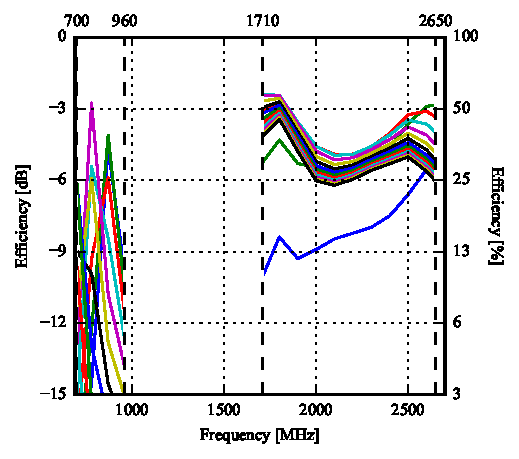
\includegraphics{img/tech_sol/nonresonant/simulation/play_mode/EffSweepAC2/efficiency-ac2-side}
        \caption{Side antenna. Sweeping $s\_C_{h1}$, fixing $C_{l3}$.}
    \end{subfigure}
    \caption{The antenna in play mode. Efficiency for each antenna when sweeping the tuning capacitors. Here, $C_{l3}$ and $s\_C_{h1}$ are the tuning capacitor for the top and side antenna, respectively.}
    \label{fig:eff_sol3play}
\end{figure}

\FloatBarrier
\subsection{Talk Mode}
Figure~\ref{fig:ant3_sparam_talk} shows the S-parameters with the tunabale capacitors set to their maxima. Such both the top and side antennas have been tuned down to the lowest possible frequency. It is seen that the top antenna covers most of the band from \SI{700}{MHz} to \SI{960}{MHz}, with a reflection coefficient below \SI{-6}{dB}. The side antenna is however very narrow band, and must be tuned in order to cover all the low bands. It is also seen that the side antenna does not cover the entire high band, when tuned down to the lowest. 

The S-parameters, when sweeping the tunable capacitors, are shown in Figure~\ref{fig:ant3_sparam_sweep_tlay}. The maximum impedance-bandwidths are summed up in Table~\ref{tab:bw_sol3data}. From this it is again clear that only the top antenna is able to cover the high end of the low band. Both antennas should be able to cover the entire high band at \SI{6}{dB} return loss.

The correlation between the antennas, when sweeping the tunable capacitors, are shown in Figure~\ref{fig:corr_sol3_tlay}. The correlation is, for frequencies above \SI{700}{MHz}, below 0.7 when sweeping the top and side antenna. For the high band the correlation is significantly lower, which is also to be expected. Again the correlation has dropped a lot from the free-space simulation in Figure~\ref{fig:corr_sol3}.

The efficiencies for each antenna, when sweeping the tuning capacitors, are shown in Figure~\ref{fig:eff_sol3talk}. It is seen that the efficiency, generally, has decreased from the free space simulation in Chapter~\ref{cha:nousersim} and also lower than the data mode. At \SI{-3}{dB} efficiency, there is no bandwidth left. At \SI{-9}{dB} most of the bands are covered.


\begin{figure}[htbp]
    \centering
    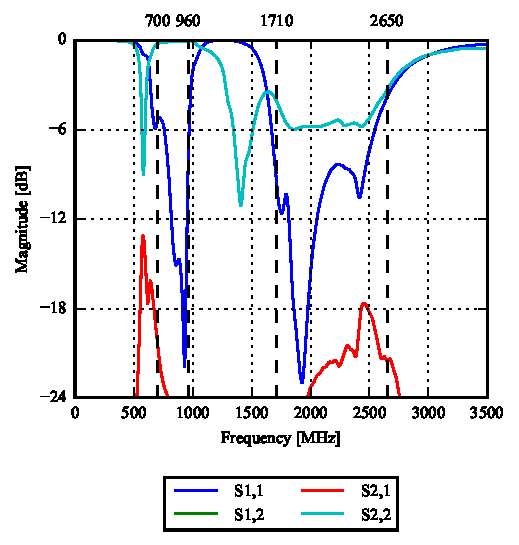
\includegraphics{img/tech_sol/nonresonant/simulation/talk_mode/s_params_cMax.pdf}
    \caption{The antenna in talk mode. S-parameters with both tuning capacitors fixed at \SI{2.9}{pF}.}
    \label{fig:ant3_sparam_talk}
\end{figure}

\begin{table}[htbp]
    \centering
    \begin{tabular}{|l|l|r|r|r|}
        \hline
        Antenna & Band & Start [MHz] & Stop [MHz] & Bandwidth [MHz] \\
        \hline
        Top     & Low  & 701         & 2597       & 1896 \\
        Side    & Low  & 749         & 844        & 95   \\
        \hline
        Top     & High & 701         & 2597       & 1896 \\
        Side    & High & 1439        & 2516       & 1077 \\
        \hline
    \end{tabular}
    \caption{The antenna in talk mode. Maximum bandwidth obtained in the low and high band for the top and the side antenna, respectively. It is, again, seen that both the low and high band are covered at the same time for the top antenna.}
    \label{tab:bw_sol3talk}
\end{table}

\begin{figure}[htbp]
   \begin{subfigure}[b]{0.49\linewidth}
        \centering
        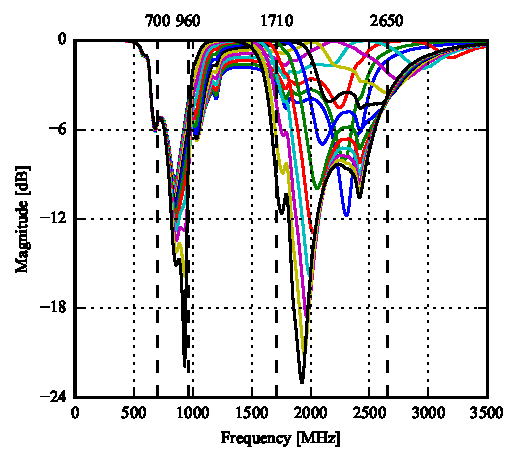
\includegraphics{img/tech_sol/nonresonant/simulation/talk_mode/s11_top_sweep.pdf}
        \caption{$S_{11}$, sweeping $C_{l3}$ and fixing $s\_C_{h1}$.}
    \end{subfigure}
    \hfill
    \begin{subfigure}[b]{0.49\linewidth}
        \centering
        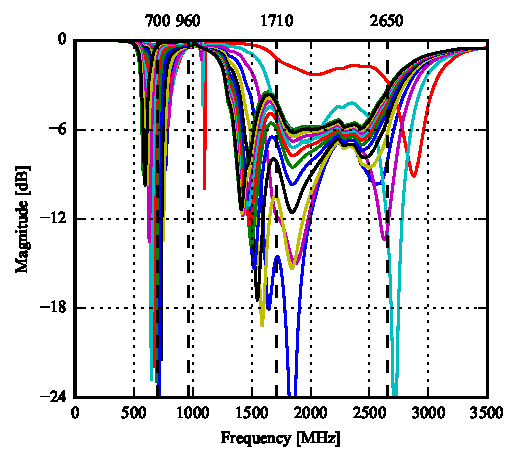
\includegraphics{img/tech_sol/nonresonant/simulation/talk_mode/s22_side_sweep.pdf}
        \caption{$S_{22}$, sweeping $C_{l3}$ and fixing $s\_C_{h1}$.}
    \end{subfigure}
    \\
    \begin{subfigure}[b]{0.49\linewidth}
        \centering
        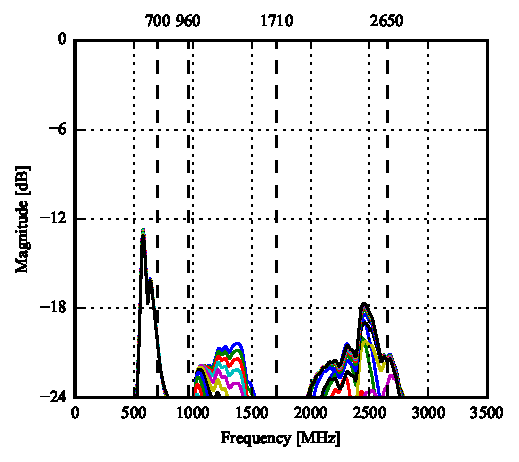
\includegraphics{img/tech_sol/nonresonant/simulation/talk_mode/s12_top_sweep.pdf}
        \caption{$S_{21}$, sweeping $C_{l3}$ and fixing $s\_C_{h1}$.}
    \end{subfigure}
    \hfill
    \begin{subfigure}[b]{0.49\linewidth}
        \centering
        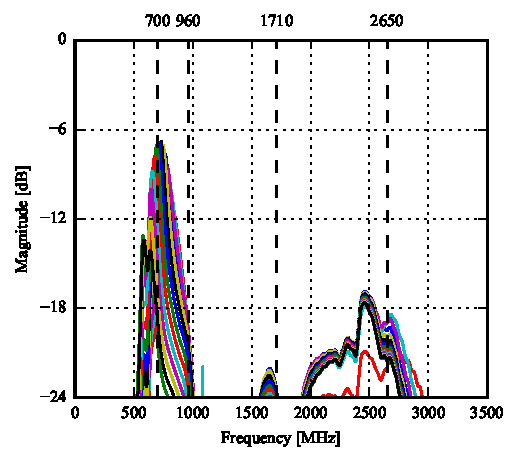
\includegraphics{img/tech_sol/nonresonant/simulation/talk_mode/s21_side_sweep.pdf}
        \caption{$S_{21}$, sweeping $s\_C_{h1}$ and fixing $C_{l3}$.}
    \end{subfigure}
    \caption{The antenna in talk mode. Parameter sweep for tuning the shunt capacitor of each antenna, $C_{l3}$ and $s\_C_{h1}$ for port 1 and 2, respectively. Port 1 is the top antenna and port 2 is the side antenna.}
    \label{fig:ant3_sparam_sweep_talk}
\end{figure}

% Correlation
\begin{figure}[htbp]
    \centering
    \begin{subfigure}{0.49\linewidth}
        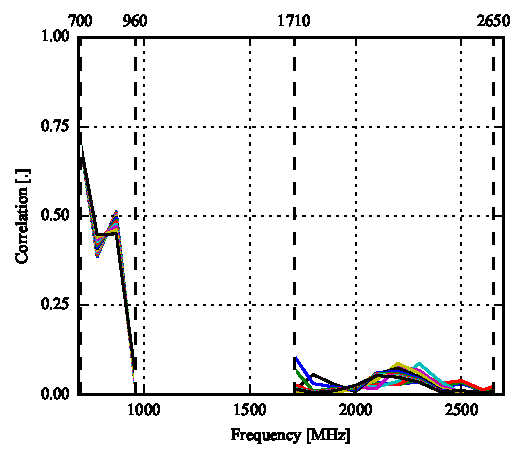
\includegraphics{img/tech_sol/nonresonant/simulation/talk_mode/sweep_top_corr}
        \caption{Sweeping $C_{l3}$ and fixing $s\_C_{h1}$.}
    \end{subfigure}
    \hfill
    \begin{subfigure}{0.49\linewidth}
        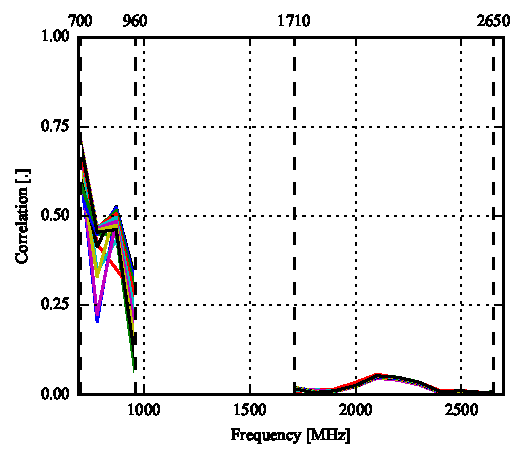
\includegraphics{img/tech_sol/nonresonant/simulation/talk_mode/sweep_side_corr}
        \caption{Sweeping $s\_C_{h1}$ and fixing $C_{l3}$.}
    \end{subfigure}
    \caption{The antenna in talk mode. Correlation between antennas then sweeping tuning capacitors. Here, $C_{l3}$ and $s\_C_{h1}$ are the tuning capacitor for the top and side antenna, respectively.}
    \label{fig:corr_sol3_talk}
\end{figure}

% Efficiency
\begin{figure}[htbp]
    \centering
    \begin{subfigure}{0.49\linewidth}
        \centering
        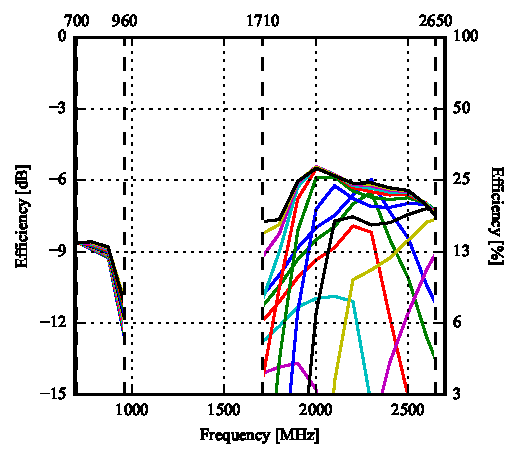
\includegraphics{img/tech_sol/nonresonant/simulation/talk_mode/EffSweepAC1/efficiency-ac1-top}
        \caption{Top antenna. Sweeping $C_{l3}$, fixing $s\_C_{h1}$.}
    \end{subfigure}
    \hfill
    \begin{subfigure}{0.49\linewidth}
        \centering
        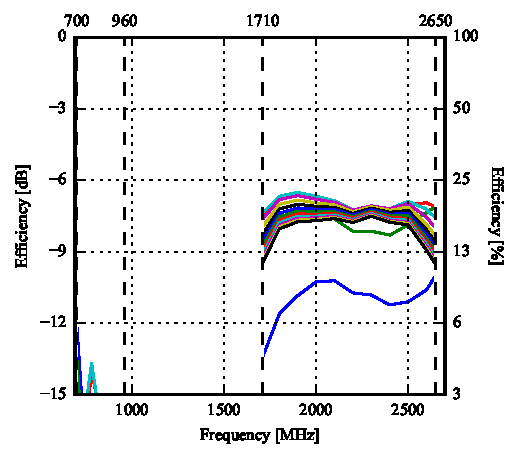
\includegraphics{img/tech_sol/nonresonant/simulation/talk_mode/EffSweepAC2/efficiency-ac2-side}
        \caption{Side antenna. Sweeping $s\_C_{h1}$, fixing $C_{l3}$.}
    \end{subfigure}
    \caption{The antenna in talk mode. Efficiency for each antenna when sweeping the tuning capacitors. Here, $C_{l3}$ and $s\_C_{h1}$ are the tuning capacitor for the top and side antenna, respectively.}
    \label{fig:eff_sol3talk}
\end{figure}


\FloatBarrier
\subsection{SAR}

The result from the SAR simulation is shown in Figure~\ref{fig:ant3_sar_sim}. It is seen, that the maximum is around \SI{1.2}{.}, which is within the maximum of \SI{2}{W\per kg} for the side antenna. A possible way to improve this may be to simulate the phone's screen, which will be located between (part of) the antenna and the head. This may reflect some of the radiated power away from the user, lowering the maximum SAR. However since it already complies with the requirements, this has not been done. 

\begin{figure}[htbp]
    \centering
    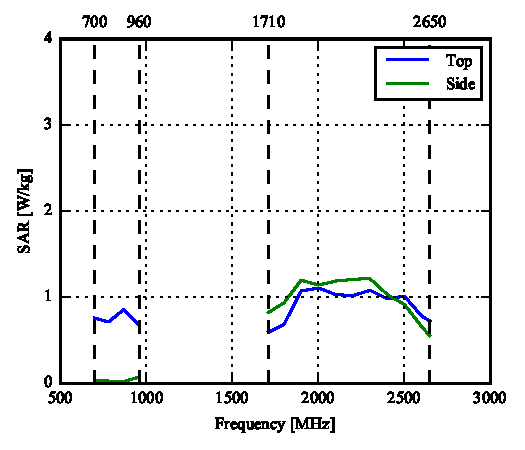
\includegraphics{img/tech_sol/nonresonant/simulation/sar/Sar_top_side.pdf}
    \caption{SAR simulation of the antenna.}
    \label{fig:ant3_sar_sim}
\end{figure}



